\section{基准U-Net模型设计与实现}

\subsection{数据集准备与预处理}

图~\ref{fig:dataset} 展示了本研究所使用的三个医学图像分割数据集中的典型图像样本:ISIC皮肤镜影像数据集、LiTS肝脏CT数据集和BraTS脑肿瘤数据集。


\begin{figure}[htbp]
    \centering
    \subfloat[皮肤镜图像(ISIC)]
    {
        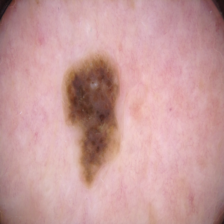
\includegraphics[width=0.3\textwidth,height=5cm]{fig/ISIC.png}
    }
    \hspace{0.3cm}
    \subfloat[肝脏CT影像(LiTS)]
    {
        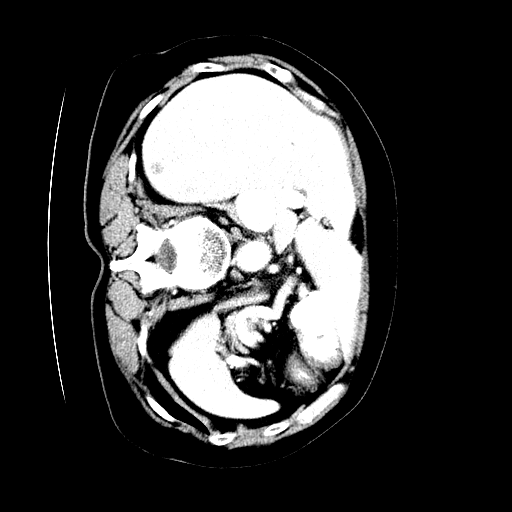
\includegraphics[width=0.3\textwidth,height=5cm]{fig/LiTS.png}
    }
    \hspace{0.3cm}
    \subfloat[脑部MRI图像(BraTS)]
    {
        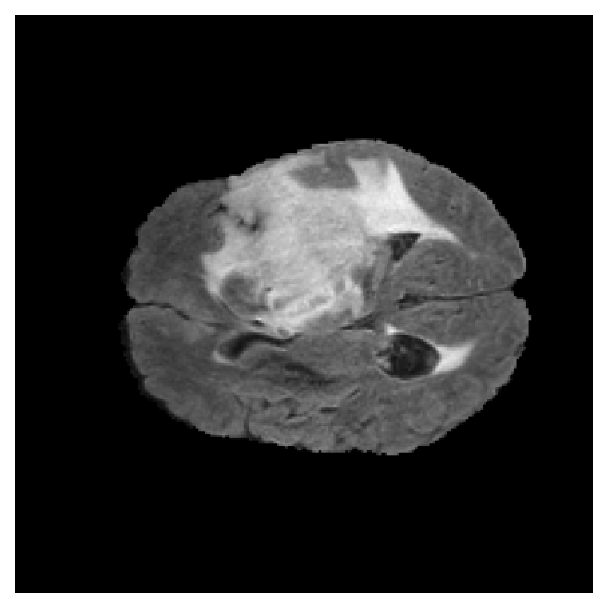
\includegraphics[width=0.3\textwidth,height=5cm]{fig/brain.pdf}
    }
    \caption{ISIC、LiTS与BraTS数据集中的典型样本图像}
    \label{fig:dataset}
\end{figure}

\subsubsection{ISIC皮肤镜影像数据集}

ISIC皮肤镜影像数据集(2018年)由ISIC联合Memorial Sloan Kettering Cancer Center、University of Queensland等多家机构共同构建,并作为ISIC 2018皮肤病变识别挑战赛的官方数据资源\cite{codella2019skinlesionanalysismelanoma}。

ISIC 2018数据集作为目前最具影响力的皮肤镜数据集之一,广泛用于皮肤病变分割模型的基准测试。数据集总共包含2594张RGB三通道皮肤镜图像,图像格式为JPEG或PNG,分辨率在600×450至6748×4499像素之间,保留了丰富的病变细节特征。在标注方面,数据集提供由皮肤科专家精确勾画的像素级病变掩膜用于病变区域分割任务训练,掩膜的标注一致性通过交叉验证确认(Kappa 系数大于 0.82)。同时,整个数据集按照任务需求被官方划分为了训练集(2,000 张,含掩膜和标签)、验证集(300 张,仅标签)与测试集(294 张,无公开标注,仅用于模型评估)。

\subsubsection{LiTS肝脏CT数据集}

LiTS(Liver Tumor Segmentation)数据集是由MICCAI 2017肝脏肿瘤分割挑战赛(Liver Tumor Segmentation Challenge 2017)发布的医学影像公开数据集,由来自全球多家权威医疗机构提供的腹部增强CT扫描组成,涵盖130例临床病例,包含多种肝脏病理状态,包括肝细胞癌、转移性肿瘤、胆管细胞癌等\cite{Bilic_2023}。所有图像数据均采用静脉期CT成像,层厚范围为1–5mm,横断面矩阵分辨率为512×512,体素间距在0.6–1.0 mm之间。

在标注方面,数据集中每一病例均由三位经验丰富的放射科专家进行独立标注,提供像素级肝脏与肿瘤分割掩膜。标注一致性通过Dice系数(平均大于0.92)和Hausdorff距离(平均小于5 mm)进行验证,部分病例还附带有病灶的病理学分型标签。

LiTS 2017数据集存在一些区别于ISIC 2018数据集的挑战:其一,肝脏轮廓复杂、变异性大,且边界常与胃肠道等邻近脏器重叠,导致区域判别困难;其二,肿瘤病灶形态异质性强(如结节型、融合型、浸润型),并存在大小悬殊、边界模糊、低密度病灶等不利因素;此外,呼吸运动伪影与层间不连续性也显著增加了分割任务的难度。

\subsubsection{BraTS脑肿瘤MRI数据集}

BraTS(Brain Tumor Segmentation)2020 数据集由 MICCAI 组织联合宾夕法尼亚大学、慕尼黑工业大学等多家国际顶尖医学与工程研究机构共同构建,作为年度脑肿瘤分割挑战赛的重要基准数据资源\cite{menze2015}。该数据集专注于胶质瘤(包括高级别胶质瘤HGG与低级别胶质瘤LGG)MRI图像的分割任务,广泛用于评估多模态影像分割算法的性能与鲁棒性。

数据集中共包含369例患者的多模态MRI扫描数据,每例数据均包含四种标准MRI模态:T1加权、T1对比增强(T1ce)、T2加权以及FLAIR。在数据标注方面,每例数据均提供由神经放射学专家联合标注的像素级三维分割掩膜,标注内容涵盖:

\begin{enumerate}
    \item 增强肿瘤区域(Enhancing Tumor,ET):表现为对比增强T1序列中具有强化表现的病灶区域;
    \item 肿瘤核心(Tumor Core,TC):包括坏死区域、实性肿瘤与增强部分;
    \item 肿瘤整体(Whole Tumor,WT):包括肿瘤核心与周围水肿区域。
\end{enumerate}

BraTS 2020数据集的主要挑战包括:(1)肿瘤组织的高度异质性,如增强区与坏死区边界模糊;(2)小体积或卫星灶的检测难度高,极易被误判或遗漏;(3)多模态之间的病灶表征差异显著,对模型特征融合能力提出更高要求。


\subsection{跨数据集标准化数据预处理}

为构建统一、可复现的医学图像分割数据管线,本文针对ISIC 2018、LiTS 2017及BraTS 2020三组数据集设计了标准化预处理框架。

所有图像数据均通过强度归一化消除跨模态差异:皮肤镜与MRI采用通道级归一化(各通道独立计算均值和方差),CT数据则通过HU值截断(LiTS限定为[-50, 400])后线性映射至[0,1]范围,以抑制无关组织干扰。数据划分采用固定随机种子的分层抽样策略,按7:2:1比例分配训练集、验证集与测试集,分层依据包括病变类型(ISIC)、肿瘤体积(LiTS)及胶质瘤级别(BraTS),划分结果持久化为JSON文件以避免数据泄漏和恢复训练的依据。标签处理上,单通道掩膜统一转换为双通道one-hot编码(背景与前景概率),适配交叉熵与Dice损失函数。  

此外,有研究表明对于脑肿瘤语义分割任务,FLAIR和T1ce这两种模态组合作为输入序列是最佳的组合选择\cite{buchner2023}。因此,针对BraTS 2020数据集,本研究仅采用FLAIR和T1ce两种模态作为输入序列,同时剔除无标注信息的空白切片以缓解类别极端不平衡问题。

该标准化的数据集处理框架在保留诊断关键信息的前提下,实现了跨模态强度可比性、解剖结构空间一致性与监督信号语义清晰度的协同优化,为后续模型的高效训练与稳定泛化奠定了数据基础。

\subsection{基准U-Net模型构建}

本研究在经典U-Net框架的基础上实现了基准U-Net模型的构建,用以评估后续改进策略的真实收益。模型构建包括网络层的搭建、损失函数的涉及和优化器的选择。

\subsubsection{网络层}

图~\ref{fig:unet_ushape}展示了本研究搭建的基准U-Net模型架构,采用对称的编码器—解码器结构:

编码端连续堆叠四级特征抽取单元,每一级由两层3×3有填充卷积与ReLU激活组成;特征通道数以32为起始,在每次下采样后按2倍的倍率递增(即32→64→128→256)。空间下采样通过2×2最大池化实现,使特征图尺寸依次减半,从而在更大的感受野上编码语义信息。

解码端采用与编码端对称的结构,对最深层特征进行转置卷积上采样,并与对应级别的编码器输出通过跳跃连接进行特征级串接后,经过两个卷积层进行卷积以还原局部细节。最终输出层采用1×1卷积,将通道数映射为像素的语义类别数后得到输出。

\begin{figure}[h]
    \centering
    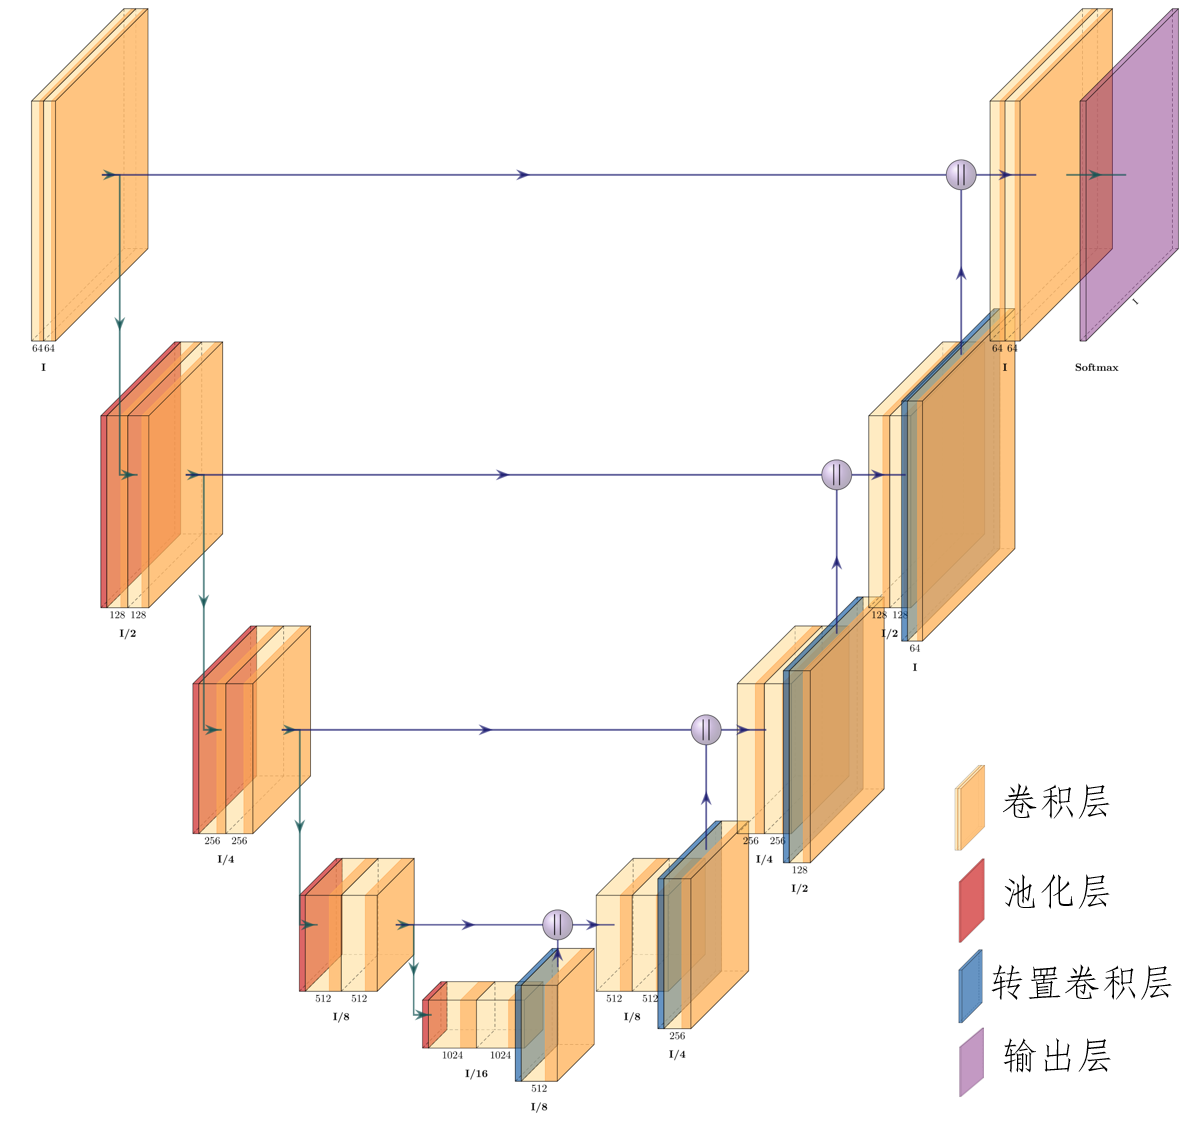
\includegraphics[width=0.6\textwidth]{fig/Unet_ushape.png}
    \caption{基准U-Net模型架构}
    \label{fig:unet_ushape}
\end{figure}

\subsubsection{损失函数的设计}

在损失函数的设计上,本文采用Dice和Cross-Entropy的混合损失函数,即以相等权重线性叠加Dice损失与像素级交叉熵(CE)损失,以充分兼顾类别不平衡下的区域重叠度优化与梯度稳定性。设网络输出的类别概率图(像素总数为$N$)为:$ P=\left\{p_{i}\right\}_{i=1}^{N} $,真实分割掩膜为$ G=\left\{g_{i}\right\}_{i=1}^{N} $,其中$ p_{i} \in[0,1], g_{i} \in\{0,1\}$分别是像素$i$的前景概率和真实标签。则:

\begin{equation}
    \mathcal{L}_{\text {Dice }}=1-\frac{2 \sum_{i=1}^{N} p_{i} g_{i}}{\sum_{i=1}^{N} p_{i}+\sum_{i=1}^{N} g_{i}+\varepsilon}
\end{equation}

\begin{equation}
    \mathcal{L}_{\mathrm{CE}}=-\frac{1}{N} \sum_{i=1}^{N}\left[g_{i} \ln \left(p_{i}\right)+\left(1-g_{i}\right) \ln \left(1-p_{i}\right)\right]
\end{equation}

\begin{equation}
    \mathcal{L}_{\text {mix }}=0.5 \mathcal{L}_{\text {Dice }}+0.5 \mathcal{L}_{\mathrm{CE}}
\end{equation}

其中$ \varepsilon=10^{-6} $用于数值平滑以防零分母。Dice项直接对预测与标注的重叠区域进行归一化度量,能在小体积病灶场景下显著提升召回;交叉熵项则提供像素级对数似然的密集监督,改善早期训练阶段梯度稀疏、收敛震荡等问题。

\subsubsection{优化器的选择}

本研究采用Adam优化器作为所有模型训练时的优化器。Adam优化器(Adaptive Moment Estimation)作为一种结合动量梯度下降与RMSprop优点的自适应学习率算法,在医学图像分割任务中展现出显著优势。其核心机制通过动态维护一阶矩估计(动量项)和二阶矩估计(自适应项)实现参数学习率的差异化调整,一阶矩平滑历史梯度方向以加速收敛:

\begin{equation}
    m_t = \beta_1 m_{t-1} + (1 - \beta_1) g_t
\end{equation}

其中,$m_t$为当前时间步的一阶矩估计,$\beta_1$是一阶矩衰减率,$g_t$为当前时间步的梯度值。

二阶矩则通过自适应缩放梯度幅度以抑制噪声干扰:

\begin{equation}
    v_t = \beta_2 v_{t-1} + (1 - \beta_2) g_t^2
\end{equation}

其中,$v_t$为当前时间步的二阶矩估计,$\beta_2$是二阶矩衰减率,$g_t^2$为当前梯度的平方。

最终通过偏差校正的更新规则,平衡探索与收敛效率:

\begin{equation}
    \theta_{t+1} = \theta_t - \eta \cdot \hat{m}_t / (\sqrt{\hat{v}_t} + \epsilon)
\end{equation}

其中,$\theta_{t+1}$表示更新后的模型参数,$\eta$是初始学习率。

相较于传统优化器,Adam在医学任务中具备多重优势:其一,自适应学习率机制可自动适配多模态数据(如MRI的T1/T2/FLAIR)的特征分布差异,避免手动调参的复杂性;其二,动量项(\( \beta_1=0.9 \))与梯度平方衰减(\( \beta_2=0.999 \))协同作用,既能抑制CT金属伪影或超声斑点噪声引发的梯度异常,又能防止学习率过早衰减;其三,初始学习率(\( \eta=1.0 \times 10^{-4} \))的精细设定兼顾了医学图像中小目标分割(如肿瘤核心)的敏感性需求与训练稳定性。实验表明,Adam在BraTS等权威挑战赛中被超过70\%的优胜模型采用,例如3D U-Net通过Adam优化使肝脏肿瘤分割的Dice系数提升4.2\%,训练周期缩短30\%,验证了其在复杂解剖结构建模中的高效性。本研究采用该优化器,旨在通过其噪声鲁棒性与自适应特性,精准捕捉病灶边界的细微差异,同时避免因局部梯度震荡导致的模型发散,为多模态医学影像的精细化分割提供可靠优化基础。

\subsection{训练策略与评估指标}

\subsubsection{训练策略}

为避免训练停滞,本研究采用动态学习率调整策略(Reduce-on-Plateau):若验证集指标连续10个epoch未提升,学习率衰减为原值的50\%,下限设为$1 \times 10^{-6}$以防止数值下溢。

而训练的批量大小则根据数据集的规模和大小以及显卡内存利用率决定,完整的训练周期设置为100epoch,且保证验证过程与训练同步。在每个epoch结束后立即于验证集评估Dice系数并记录最优权重;测试集仅使用单尺度推断,不采用多尺度或模型集成,确保基准模型公平、简洁、可复现。

\subsubsection{评估指标}

在医学图像分割研究中,模型输出通常为与输入图像同尺寸的二值概率图,衡量其与专家标注掩膜之间的相似程度是评价算法优劣的关键。单一指标无法满足同时反映检测率、误诊率和重叠精度的要求,多指标可立体呈现模型表现。

本研究以混淆矩阵四要素(真阳性TP、真阴性TN、假阳性FP、假阴性FN)为基础,记录Accuracy、Precision、Recall、Specificity、F1-Score、Dice系数与Jaccard指数七项评估指标。下文将逐一给出这些指标的定义、公式及其评价意义。

准确率Accuracy表示正确预测的样本占总样本的比例,是最直观的分类性能指标:

\begin{equation}
    \mathrm{Accuracy}=\frac{TP+TN}{TP+TN+FP+FN}
\end{equation}

Accuracy直观反映模型的综合判断能力,但在病灶面积远小于背景时,Accuracy易受TN主导,可能高估模型质量,因此仅作为参考基线。

特异性Specificity表示实际为负类的样本中被正确预测的比例,衡量模型识别阴性样本的能力:

\begin{equation}
    \mathrm{Specificity}=\frac{T N}{T N+F P}
\end{equation}

在医学任务中,高特异性可减少健康组织被误判为病变的风险(如避免正常脑组织被误分割为肿瘤),提升结果的可信度,与 Recall 形成互补。

Jaccard指数(IoU)计算预测与真实标签的交集与并集的比值,是分割任务的经典指标:

精确率Precision表示预测为正类的样本中实际为正类的比例,反映模型的预测可靠性:

\begin{equation}
    \mathrm{Precision}=\frac{T P}{T P+F P}
\end{equation}

Precision反映模型整体预测正确性,但在类别极度不平衡时(如背景像素占比90\%以上),可能高估性能(例如模型仅预测背景即可获得高准确率),需结合其他指标综合判断。

召回率Recall召回率表示实际为正类的样本中被正确预测的比例,反映模型对正类样本的覆盖能力:

\begin{equation}
    \mathrm{Recall}=\frac{T P}{T P+F N} 
\end{equation}

高召回率意味着模型能有效捕捉病变区域(减少漏检),在早期诊断(如癌症筛查)中至关重要,但需平衡精确率以避免过度预测。

F1-Score是Precision与Recall的调和平均数,综合衡量模型在正类样本上的分类能力,尤其适用于类别不平衡场景:

\begin{equation}
    \mathrm{F} 1=\frac{2 T P}{2 T P+F P+F N}=2 \cdot \frac{\text { Precision } \times \text { Recall }}{\text { Precision }+ \text { Recall }}
\end{equation}

F1分数可以避免仅关注单一指标(如高精确率但低召回率),在医学图像分割中(如肿瘤区域占比小),能更均衡评估模型对正类(病变区域)的捕捉能力与预测准确性。

Dice系数衡量预测结果与真实标签的重叠程度,是医学图像分割的核心评估指标:

\begin{equation}
    \mathrm{Dice}=\frac{2 T P}{2 T P+F P+F N}=\frac{2 \times|A \cap B|}{|A|+|B|}
\end{equation}

其中,A为预测区域,B为真实区域。Dice系数直接衡量空间重叠,对不平衡数据敏感度低,能有效评估模型对病灶轮廓的捕捉精度,尤其适用于小目标分割任务(如脑肿瘤核心)。

\begin{equation}
    \mathrm{Jaccard}=\frac{T P}{T P+F P+F N}=\frac{|A \cap B|}{|A \cup B|}
\end{equation}

其中,A为预测区域,B为真实区域。Jaccard指数严格量化重叠区域的比例,对分割边界的轻微偏移敏感,常用于评估模型在复杂解剖结构(如肿瘤浸润区域)中的细节保留能力,在多模型比较时可提供更保守的评估视角。